\documentclass[a4paper, 12pt]{article}

\usepackage{hyperref}
\usepackage[warn]{mathtext}
\usepackage[utf8]{inputenc}
\usepackage[T2A]{fontenc}
\usepackage[english,russian]{babel}
\usepackage{multirow}
\usepackage{amsmath,amsfonts,amssymb,amsthm,mathtools}
\usepackage{indentfirst}
\DeclareSymbolFont{T2Aletters}{T2A}{cmr}{m}{it}
\usepackage{ gensymb }
\mathtoolsset{showonlyrefs=true}
\usepackage{euscript}
\usepackage{mathrsfs}
\usepackage[left=2cm,right=2cm,top=2cm,bottom=2cm]{geometry}
\usepackage{graphicx}
\usepackage{wrapfig}
\usepackage[rgb]{xcolor}
\hypersetup{
colorlinks=true,
urlcolor=blue
}


\title{Лабораторная работа}
\author{Гисич Арсений Б03-102}
\date{2022}

\begin{document}

	\begin{center}
		{\large МОСКОВСКИЙ ФИЗИКО-ТЕХНИЧЕСКИЙ ИНСТИТУТ (НАЦИОНАЛЬНЫЙ ИССЛЕДОВАТЕЛЬСКИЙ УНИВЕРСИТЕТ)}
	\end{center}
	\vspace{5 cm}
	{\Large
		\begin{center}
			{\bf Лабораторная работа 3.4.2}\\[0.2 cm]
			Закон Кюри-Вейсса
		\end{center}
	}
	\vspace{4 cm}
	\begin{flushright}
		{\Large Выполнил: \\
			\vspace{0.2 cm}
			Гисич Арсений \\
			\vspace{0.2 cm}
			Б03-102 \\}
	\end{flushright}
	\vspace{9 cm}
	\begin{center}
		Долгопрудный\\[0.1 cm]
		2022
	\end{center}
\thispagestyle{empty}

\section{Аннотация}

В данной работе проводится исследование зависимости магнитной восприимчивости гадолиния, который является ферромагнетиком, от температуры. Исследование приведено для температур от 14 до 40 \textcelsius. На основании этой зависимости вычисляется точка Кюри гадолиния.

\section{Теоретические сведения}

Вещества с отличными от нуля атомными магнитными моментами обладают парамагнитными свойствами. Внешнее магнитное поле ориентирует магнитные моменты, которые в отсутствие поля располагались в пространстве хаотическим образом. Однако при $T \rightarrow 0$ тепловое движение всё меньше препятствует магнитным моментам атомов ориентироваться в одном направлении при сколь угодно слабом внешнем поле. В ферромагнетиках -- под влиянием обменных сил -- это происходит при понижении температуры не до абсолютного нуля, а до температуры Кюри $\Theta$. Оказывается, что у ферромагнетиков магнитная восприимчивость должна удовлетворять закону Кюри-Вейсса:
\begin{equation}
	\label{eq:Kuri-Veicca}
	\chi \propto \frac{1}{T-\Theta_p},
\end{equation}
где $\Theta_p$ -- температура, близкая к температуре Кюри, так как при $T \approx \Theta$ формула~(\ref{eq:Kuri-Veicca}) недостаточна точна.

\section{Методика измерений}

Экспериментальная установка. Схема установки для проверки Закона Кюри-Вейсса показана на рис.~\ref{ris1}. Исследуемый ферромагнитный образец (гадолиний) расположен внутри пустотелой катушки самоиндукции, которая служит индуктивностью колебательного контура, входящего в состав $L C$ -автогенератора.

\begin{figure}[h!]
\begin{center}
    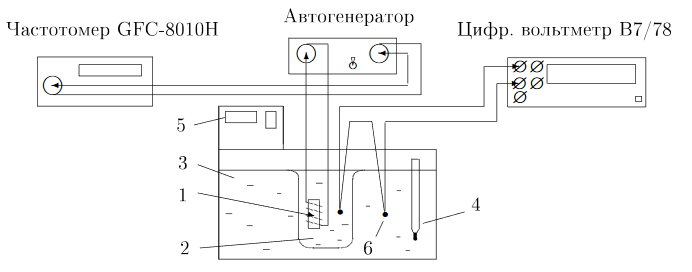
\includegraphics[scale=0.8]{1.png}
\end{center}
\caption{Схема экспериментальной установки}
\label{ris1}
\end{figure}

Гадолиний является хорошим проводником электрического тока, a paбoчая частота генератора достаточно велика $(\sim 50$ кГц $),$ поэтому для уменьшения вихревых токов образец изготовлен из мелких кусочков размером $\sim 0,5$ мм. Катушка 1 с образцом помещена в стеклянный сосуд 2, залитый трансформаторным маслом. Масло предохраняет образец от окисления и способствует ухудшению электрического контакта между отдельными частичками образца. Кроме того, оно улучшает тепловой контакт между образцом и термостатируемой (рабочей) жидкостью 3 в термостате. Ртутный термометр 4 используется для приближённой оценки температуры. Температура образца регулируется с помощью термостата 5.

Магнитная восприимчивость образца $\chi$ определяется по изменению самоиндукции катушки. Обозначив через $L$ самоиндукцию катушки с образцом и через $L_0$ -- её самоиндукцию в отсутствие образца, получим
\begin{equation*}
	(L-L_0)\propto \chi.
\end{equation*}
При изменении самоиндукции образца меняется период колебаний автогенератора:
\begin{equation*}
	\tau = 2\pi \sqrt{LC},
\end{equation*}
где $C$ -- ёмкость контура автогенератора. Период колебаний в отсутствие образца определяется самоиндукцией пустой катушки:
\begin{equation*}
	\tau_0 = 2\pi \sqrt{L_0C}.
\end{equation*}

Итак, закон Кюри-Вейсса справедлив, если выполнено соотношение:
\begin{equation}
	\frac{1}{\chi} \propto (T-\Theta_p) \propto \frac{1}{\tau^2-\tau_0^2}.
\end{equation}

Измерения проводятся в интервале температур от 14~\textcelsius\, до 40~\textcelsius.

\section{Используемое оборудование}

\begin{enumerate}
    \item катушка самоиндукции с образцом из гадолиния;
    \item термостат;
    \item частотомер;
    \item цифровой вольтметр;
    \item $LC$-автогенератор;
    \item термопара медь-константан;
\end{enumerate}

\section{Результаты измерений и обработка данных}

\begin{table}[h!]
\begin{center}
\begin{tabular}{|c|c|c|c|c|c|c|c|c|}
\hline
$n$ & $\nu_{т}, кГц$ & $a_{т}$ & $норм(a_{т})$ & $\nu_{изм}, кГц$ & $\delta_{\nu_{изм}}, кГц$ & $a_{изм}, мВ$ & $\delta_{a_{изм}}, мВ$ & $норм(a_{изм})$ \\ \hline
1 & 1 & 144,51 & 8,81 & 1,00 & 0,02 & 820 & 2 & 8,54 \\ \hline
2 & 2 & 128,76 & 7,85 & 2,00 & 0,02 & 736 & 2 & 7,67 \\ \hline
3 & 3 & 104,80 & 6,39 & 3,00 & 0,02 & 600 & 2 & 6,25 \\ \hline
4 & 4 & 75,68 & 4,62 & 4,00 & 0,02 & 432 & 2 & 4,50 \\ \hline
5 & 5 & 45,02 & 2,75 & 5,00 & 0,02 & 264 & 2 & 2,75 \\ \hline
6 & 6 & 16,39 & 1 & 6,00 & 0,02 & 96 & 2 & 1 \\ \hline
\end{tabular}
\end{center}
\caption{Результаты теоретического расчёта и измерений амплитуд и частот первых 6 гармоник спектра}
\label{tab1}
\end{table}


\section{Обсуждение результатов и выводы}

В данной работе был исследован спектральный состав периодических электрических сигналов.

При исследовании спектра периодической последовательности прямоугольных импульсов при фиксированных параметрах $\nu_{повт}$ и $\tau$ были измерены амплитуды и частоты первых 6 гармоник (таб.~\ref{tab1}). Измеренные значения соответствуют рассчитанным теоретически. Также была измерена зависимость ширины спектра $\Delta{\nu}$ от времени импульса $\tau$. Из полученной зависимости (рис.~\ref{plot1}) следует: $$\Delta{\nu} \cdot \tau \backsimeq 1,01\pm0,01,$$ что соответствует соотношению неопределённостей в рамках погрешности. Основной вклад в погрешность вносит определение коэффициента зависимости, так как благодаря использованию цифровых приборов другие источники погрешности отсутствуют или их влияние несущественно.

При исследовании спектра периодической последовательности цугов была измерена зависимость расстояния $\delta{\nu}$ между соседними спектральными компонентами сигнала от периода $T$ повторения импульсов. Из полученной зависимости (рис.~\ref{plot2}) следует: $$\delta{\nu} \cdot \tau \backsimeq 0,95\pm0,01,$$ что близко к соотношению неопределённостей. Здесь основной вклад в погрешность также вносит определение коэффициента зависимости.

При исследовании спектра амплитудно-модулированного сигнала была измерена зависимость отношения $a_{бок}/a_{осн}$ амплитуд боковой и основной спектральных линий от глубины модуляции $m$. Из полученной зависимости (рис.~\ref{plot3}) следует: $$\frac{a_{бок}}{a_{осн}} = 0,510\pm0,004 \cdot m,$$ что соответствует теоретической зависимости $\frac{a_{бок}}{a_{осн}} = \frac{m}{2}$. Аналогично здесь основной вклад в погрешность вносит определение коэффициента зависимости.

Также в данной работе был изучен спектр сигнала, модулированного по фазе. Спектры сигналов при различном максимальном отклонении $\varphi_m$ приведены на рис.~\ref{ris24}-\ref{ris25}.

\end{document}
